\documentclass[aspectratio=169,10pt]{beamer}
\usetheme{Madrid}
\usecolortheme{whale}
\usepackage{pgfplots}
\pgfplotsset{compat=1.18}
\usepackage{booktabs}
\usepackage{amsmath}

\pgfplotsset{
  every axis/.style={
    width=6.5cm, height=5cm,
    grid=major, grid style={dashed,gray!40},
    mark size=1.5pt,
    xlabel={$p$},
    scaled ticks=false,
    xticklabel style={font=\tiny, /pgf/number format/fixed},
    yticklabel style={font=\tiny, /pgf/number format/fixed},
  },
  black line/.style={
    smooth, thick, black,
  },
}

\title{Results for presentation (model with haircut)}
\author{Hector Castillo Andreu}
\date{\today}

\begin{document}

\begin{frame}
  \titlepage
\end{frame}

\begin{frame}{Bankruptcies}
  \begin{columns}[T]
    \begin{column}{0.4\textwidth}
      \centering
      \small $p=[0 .. 1]$\\
      \begin{figure}
        \centering
        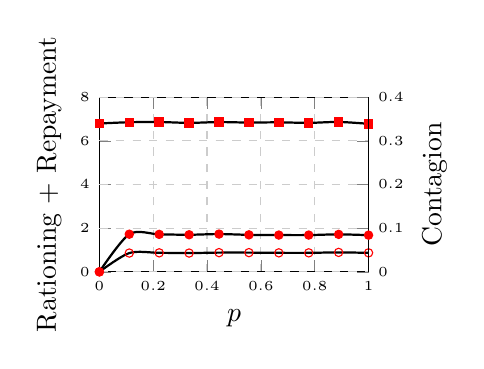
\begin{tikzpicture}
        \begin{axis}[
          ylabel={Rationing + Repayment},
          ymin=0, ymax=8,
          xmin=0, xmax=1.0,
          width=5cm, height=3.8cm,
        ]
          \addplot[only marks, mark=square*, red] coordinates { (1e-05,6.7930) (0.11112,6.8513) (0.22223,6.8612) (0.33334,6.8222) (0.44445,6.8584) (0.5555599999999999,6.8366) (0.66667,6.8472) (0.7777799999999999,6.8218) (0.88889,6.8642) (1.0,6.7793) };
          \addplot[black line] coordinates { (1e-05,6.7930) (0.11112,6.8513) (0.22223,6.8612) (0.33334,6.8222) (0.44445,6.8584) (0.5555599999999999,6.8366) (0.66667,6.8472) (0.7777799999999999,6.8218) (0.88889,6.8642) (1.0,6.7793) };
          \addplot[only marks, mark=o, red] coordinates { (1e-05,0.00) (0.11112,0.86) (0.22223,0.87) (0.33334,0.86) (0.44445,0.88) (0.5555599999999999,0.88) (0.66667,0.87) (0.7777799999999999,0.87) (0.88889,0.89) (1.0,0.87) };
          \addplot[black line] coordinates { (1e-05,0.00) (0.11112,0.86) (0.22223,0.87) (0.33334,0.86) (0.44445,0.88) (0.5555599999999999,0.88) (0.66667,0.87) (0.7777799999999999,0.87) (0.88889,0.89) (1.0,0.87) };
        \end{axis}
        \begin{axis}[
          ylabel={Contagion},
          ymin=0, ymax=0.4,
          xmin=0, xmax=1.0,
          axis y line*=right, axis x line=none,
          ylabel near ticks,
          width=5cm, height=3.8cm,
        ]
          \addplot[only marks, mark=*, red] coordinates { (1e-05,0.0000) (0.11112,0.0862) (0.22223,0.0858) (0.33334,0.0849) (0.44445,0.0865) (0.5555599999999999,0.0847) (0.66667,0.0842) (0.7777799999999999,0.0842) (0.88889,0.0858) (1.0,0.0840) };
          \addplot[black line] coordinates { (1e-05,0.0000) (0.11112,0.0862) (0.22223,0.0858) (0.33334,0.0849) (0.44445,0.0865) (0.5555599999999999,0.0847) (0.66667,0.0842) (0.7777799999999999,0.0842) (0.88889,0.0858) (1.0,0.0840) };
        \end{axis}
        \end{tikzpicture}
      \end{figure}
      \vspace{-0.3cm}
      \tiny\renewcommand{\arraystretch}{0.85}\setlength{\tabcolsep}{2pt}
      \centering
      \begin{tabular}{@{}l@{\hspace{0.3cm}}l@{}}
        \begin{tabular}{lccc}
          \toprule
          $p$ & Rat. & Cont. & Fail. \\
          \midrule
          0.00001 & 6.79 & 0.00 & 0.00 \\
          0.111 & 6.85 & 0.09 & 0.86 \\
          0.222 & 6.86 & 0.09 & 0.87 \\
          0.333 & 6.82 & 0.08 & 0.86 \\
          0.444 & 6.86 & 0.09 & 0.88 \\
          0.556 & 6.84 & 0.08 & 0.88 \\
          0.667 & 6.85 & 0.08 & 0.87 \\
          0.778 & 6.82 & 0.08 & 0.87 \\
          0.889 & 6.86 & 0.09 & 0.89 \\
          1.000 & 6.78 & 0.08 & 0.87 \\
          \bottomrule
        \end{tabular}
        &
        \begin{tabular}{l}
          \textcolor{red}{$\blacksquare$} Rationing \\
          \textcolor{red}{$\circ$} Failed \\
          \textcolor{red}{$\bullet$} Contagion
        \end{tabular}
      \end{tabular}
    \end{column}
    \begin{column}{0.6\textwidth}
      \centering
      \small $p=[0 .. 0.12]$\\
      \begin{figure}
        \centering
        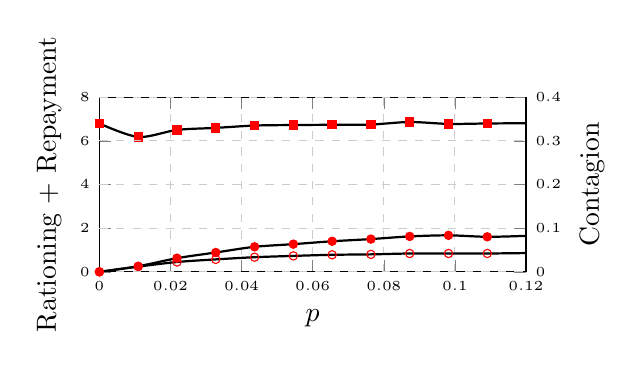
\begin{tikzpicture}
        \begin{axis}[
          ylabel={Rationing + Repayment},
          ymin=0, ymax=8,
          xmin=0, xmax=0.12,
          width=7cm, height=3.8cm,
        ]
          \addplot[only marks, mark=square*, red] coordinates { (1e-05,6.7931) (0.01091909090909091,6.1768) (0.02182818181818182,6.4994) (0.03273727272727273,6.5926) (0.04364636363636364,6.6995) (0.05455545454545455,6.7234) (0.06546454545454546,6.7342) (0.07637363636363637,6.7453) (0.08728272727272728,6.8621) (0.09819181818181819,6.7748) (0.1091009090909091,6.7942) (0.12001,6.8065) };
          \addplot[black line] coordinates { (1e-05,6.7931) (0.01091909090909091,6.1768) (0.02182818181818182,6.4994) (0.03273727272727273,6.5926) (0.04364636363636364,6.6995) (0.05455545454545455,6.7234) (0.06546454545454546,6.7342) (0.07637363636363637,6.7453) (0.08728272727272728,6.8621) (0.09819181818181819,6.7748) (0.1091009090909091,6.7942) (0.12001,6.8065) };
          \addplot[only marks, mark=o, red] coordinates { (1e-05,0.00) (0.01091909090909091,0.24) (0.02182818181818182,0.45) (0.03273727272727273,0.57) (0.04364636363636364,0.67) (0.05455545454545455,0.73) (0.06546454545454546,0.78) (0.07637363636363637,0.80) (0.08728272727272728,0.84) (0.09819181818181819,0.84) (0.1091009090909091,0.84) (0.12001,0.86) };
          \addplot[black line] coordinates { (1e-05,0.00) (0.01091909090909091,0.24) (0.02182818181818182,0.45) (0.03273727272727273,0.57) (0.04364636363636364,0.67) (0.05455545454545455,0.73) (0.06546454545454546,0.78) (0.07637363636363637,0.80) (0.08728272727272728,0.84) (0.09819181818181819,0.84) (0.1091009090909091,0.84) (0.12001,0.86) };
        \end{axis}
        \begin{axis}[
          ylabel={Contagion},
          ymin=0, ymax=0.4,
          xmin=0, xmax=0.12,
          axis y line*=right, axis x line=none,
          ylabel near ticks,
          width=7cm, height=3.8cm,
        ]
          \addplot[only marks, mark=*, red] coordinates { (1e-05,0.0000) (0.01091909090909091,0.0128) (0.02182818181818182,0.0313) (0.03273727272727273,0.0443) (0.04364636363636364,0.0573) (0.05455545454545455,0.0634) (0.06546454545454546,0.0700) (0.07637363636363637,0.0750) (0.08728272727272728,0.0811) (0.09819181818181819,0.0836) (0.1091009090909091,0.0802) (0.12001,0.0824) };
          \addplot[black line] coordinates { (1e-05,0.0000) (0.01091909090909091,0.0128) (0.02182818181818182,0.0313) (0.03273727272727273,0.0443) (0.04364636363636364,0.0573) (0.05455545454545455,0.0634) (0.06546454545454546,0.0700) (0.07637363636363637,0.0750) (0.08728272727272728,0.0811) (0.09819181818181819,0.0836) (0.1091009090909091,0.0802) (0.12001,0.0824) };
        \end{axis}
        \end{tikzpicture}
      \end{figure}
      \vspace{-0.3cm}
      \tiny\renewcommand{\arraystretch}{0.85}\setlength{\tabcolsep}{2pt}
      \centering
      \begin{tabular}{@{}l@{\hspace{0.3cm}}l@{}}
        \begin{tabular}{lccc}
          \toprule
          $p$ & Rat. & Cont. & Fail. \\
          \midrule
          0.00001 & 6.79 & 0.00 & 0.00 \\
          0.011 & 6.18 & 0.01 & 0.24 \\
          0.022 & 6.50 & 0.03 & 0.45 \\
          0.033 & 6.59 & 0.04 & 0.57 \\
          0.044 & 6.70 & 0.06 & 0.67 \\
          0.055 & 6.72 & 0.06 & 0.73 \\
          0.065 & 6.73 & 0.07 & 0.78 \\
          0.076 & 6.75 & 0.07 & 0.80 \\
          0.087 & 6.86 & 0.08 & 0.84 \\
          0.098 & 6.77 & 0.08 & 0.84 \\
          0.109 & 6.79 & 0.08 & 0.84 \\
          0.120 & 6.81 & 0.08 & 0.86 \\
          \bottomrule
        \end{tabular}
        &
        \begin{tabular}{l}
          \textcolor{red}{$\blacksquare$} Rationing \\
          \textcolor{red}{$\circ$} Failed \\
          \textcolor{red}{$\bullet$} Contagion
        \end{tabular}
      \end{tabular}
    \end{column}
  \end{columns}
\end{frame}

\begin{frame}{Loans }
  \begin{columns}[T]
    \begin{column}{0.4\textwidth}
      \centering
      \small $p=[0 .. 1]$\\
      \begin{figure}
        \centering
        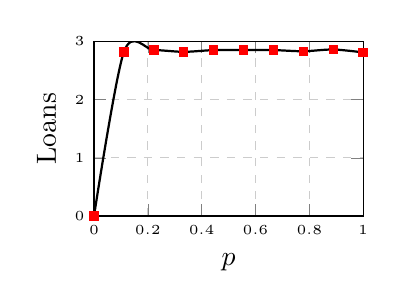
\begin{tikzpicture}
        \begin{axis}[
          ylabel={Loans},
          ymin=0,
          xmin=0, xmax=1.0,
          width=5cm, height=3.8cm,
          ymax=3,
        ]
          \addplot[only marks, mark=square*, red] coordinates { (1e-05,0.00) (0.11112,2.82) (0.22223,2.85) (0.33334,2.82) (0.44445,2.85) (0.5555599999999999,2.85) (0.66667,2.85) (0.7777799999999999,2.83) (0.88889,2.86) (1.0,2.81) };
          \addplot[black line] coordinates { (1e-05,0.00) (0.11112,2.82) (0.22223,2.85) (0.33334,2.82) (0.44445,2.85) (0.5555599999999999,2.85) (0.66667,2.85) (0.7777799999999999,2.83) (0.88889,2.86) (1.0,2.81) };
        \end{axis}
        \end{tikzpicture}
      \end{figure}
      \vspace{-0.3cm}
      \tiny\renewcommand{\arraystretch}{0.85}\setlength{\tabcolsep}{2pt}
      \centering
      \begin{tabular}{lr}
        \toprule
        $p$ & Val. \\
        \midrule
          0.00001 & 0.00 \\
          0.111 & 2.82 \\
          0.222 & 2.85 \\
          0.333 & 2.82 \\
          0.444 & 2.85 \\
          0.556 & 2.85 \\
          0.667 & 2.85 \\
          0.778 & 2.83 \\
          0.889 & 2.86 \\
          1.000 & 2.81 \\
        \bottomrule
      \end{tabular}
    \end{column}
    \begin{column}{0.6\textwidth}
      \centering
      \small $p=[0 .. 0.12]$\\
      \begin{figure}
        \centering
        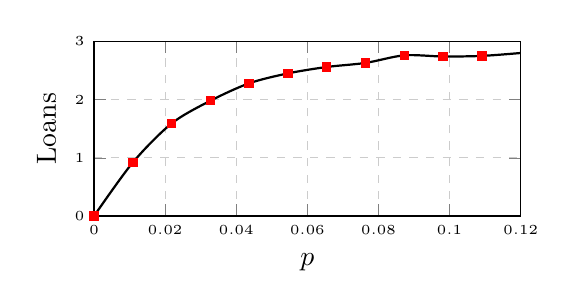
\begin{tikzpicture}
        \begin{axis}[
          ylabel={Loans},
          ymin=0,
          xmin=0, xmax=0.12,
          width=7cm, height=3.8cm,
          ymax=3,
        ]
          \addplot[only marks, mark=square*, red] coordinates { (1e-05,0.00) (0.01091909090909091,0.92) (0.02182818181818182,1.59) (0.03273727272727273,1.98) (0.04364636363636364,2.28) (0.05455545454545455,2.45) (0.06546454545454546,2.56) (0.07637363636363637,2.63) (0.08728272727272728,2.76) (0.09819181818181819,2.74) (0.1091009090909091,2.75) (0.12001,2.80) };
          \addplot[black line] coordinates { (1e-05,0.00) (0.01091909090909091,0.92) (0.02182818181818182,1.59) (0.03273727272727273,1.98) (0.04364636363636364,2.28) (0.05455545454545455,2.45) (0.06546454545454546,2.56) (0.07637363636363637,2.63) (0.08728272727272728,2.76) (0.09819181818181819,2.74) (0.1091009090909091,2.75) (0.12001,2.80) };
        \end{axis}
        \end{tikzpicture}
      \end{figure}
      \vspace{-0.3cm}
      \tiny\renewcommand{\arraystretch}{0.85}\setlength{\tabcolsep}{2pt}
      \centering
      \begin{tabular}{lr}
        \toprule
        $p$ & Val. \\
        \midrule
          0.00001 & 0.00 \\
          0.011 & 0.92 \\
          0.022 & 1.59 \\
          0.033 & 1.98 \\
          0.044 & 2.28 \\
          0.055 & 2.45 \\
          0.065 & 2.56 \\
          0.076 & 2.63 \\
          0.087 & 2.76 \\
          0.098 & 2.74 \\
          0.109 & 2.75 \\
          0.120 & 2.80 \\
        \bottomrule
      \end{tabular}
    \end{column}
  \end{columns}
\end{frame}

\begin{frame}{Bad Debt }
  \begin{columns}[T]
    \begin{column}{0.4\textwidth}
      \centering
      \small $p=[0 .. 1]$\\
      \begin{figure}
        \centering
        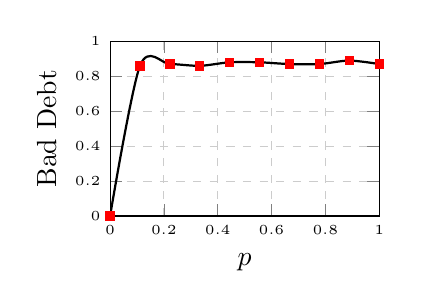
\begin{tikzpicture}
        \begin{axis}[
          ylabel={Bad Debt},
          ymin=0,
          xmin=0, xmax=1.0,
          width=5cm, height=3.8cm,
          ymax=1,
        ]
          \addplot[only marks, mark=square*, red] coordinates { (1e-05,0.00) (0.11112,0.86) (0.22223,0.87) (0.33334,0.86) (0.44445,0.88) (0.5555599999999999,0.88) (0.66667,0.87) (0.7777799999999999,0.87) (0.88889,0.89) (1.0,0.87) };
          \addplot[black line] coordinates { (1e-05,0.00) (0.11112,0.86) (0.22223,0.87) (0.33334,0.86) (0.44445,0.88) (0.5555599999999999,0.88) (0.66667,0.87) (0.7777799999999999,0.87) (0.88889,0.89) (1.0,0.87) };
        \end{axis}
        \end{tikzpicture}
      \end{figure}
      \vspace{-0.3cm}
      \tiny\renewcommand{\arraystretch}{0.85}\setlength{\tabcolsep}{2pt}
      \centering
      \begin{tabular}{lr}
        \toprule
        $p$ & Val. \\
        \midrule
          0.00001 & 0.00 \\
          0.111 & 0.86 \\
          0.222 & 0.87 \\
          0.333 & 0.86 \\
          0.444 & 0.88 \\
          0.556 & 0.88 \\
          0.667 & 0.87 \\
          0.778 & 0.87 \\
          0.889 & 0.89 \\
          1.000 & 0.87 \\
        \bottomrule
      \end{tabular}
    \end{column}
    \begin{column}{0.6\textwidth}
      \centering
      \small $p=[0 .. 0.12]$\\
      \begin{figure}
        \centering
        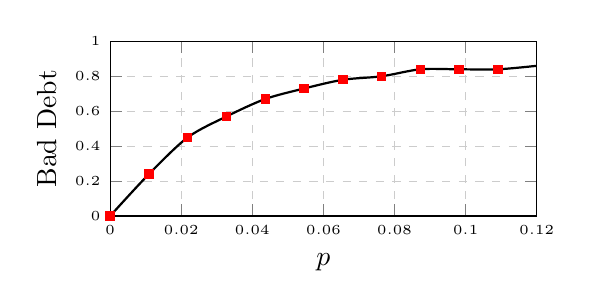
\begin{tikzpicture}
        \begin{axis}[
          ylabel={Bad Debt},
          ymin=0,
          xmin=0, xmax=0.12,
          width=7cm, height=3.8cm,
          ymax=1,
        ]
          \addplot[only marks, mark=square*, red] coordinates { (1e-05,0.00) (0.01091909090909091,0.24) (0.02182818181818182,0.45) (0.03273727272727273,0.57) (0.04364636363636364,0.67) (0.05455545454545455,0.73) (0.06546454545454546,0.78) (0.07637363636363637,0.80) (0.08728272727272728,0.84) (0.09819181818181819,0.84) (0.1091009090909091,0.84) (0.12001,0.86) };
          \addplot[black line] coordinates { (1e-05,0.00) (0.01091909090909091,0.24) (0.02182818181818182,0.45) (0.03273727272727273,0.57) (0.04364636363636364,0.67) (0.05455545454545455,0.73) (0.06546454545454546,0.78) (0.07637363636363637,0.80) (0.08728272727272728,0.84) (0.09819181818181819,0.84) (0.1091009090909091,0.84) (0.12001,0.86) };
        \end{axis}
        \end{tikzpicture}
      \end{figure}
      \vspace{-0.3cm}
      \tiny\renewcommand{\arraystretch}{0.85}\setlength{\tabcolsep}{2pt}
      \centering
      \begin{tabular}{lr}
        \toprule
        $p$ & Val. \\
        \midrule
          0.00001 & 0.00 \\
          0.011 & 0.24 \\
          0.022 & 0.45 \\
          0.033 & 0.57 \\
          0.044 & 0.67 \\
          0.055 & 0.73 \\
          0.065 & 0.78 \\
          0.076 & 0.80 \\
          0.087 & 0.84 \\
          0.098 & 0.84 \\
          0.109 & 0.84 \\
          0.120 & 0.86 \\
        \bottomrule
      \end{tabular}
    \end{column}
  \end{columns}
\end{frame}

\begin{frame}{Number of Loans }
  \begin{columns}[T]
    \begin{column}{0.4\textwidth}
      \centering
      \small $p=[0 .. 1]$\\
      \begin{figure}
        \centering
        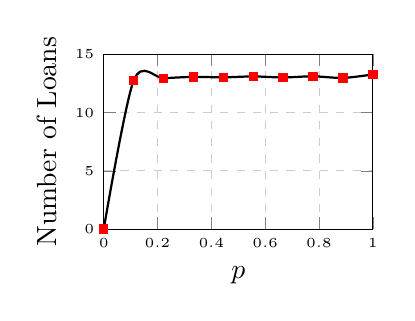
\begin{tikzpicture}
        \begin{axis}[
          ylabel={Number of Loans},
          ymin=0,
          xmin=0, xmax=1.0,
          width=5cm, height=3.8cm,
          ymax=15,
        ]
          \addplot[only marks, mark=square*, red] coordinates { (1e-05,0.00) (0.11112,12.75) (0.22223,12.95) (0.33334,13.07) (0.44445,13.03) (0.5555599999999999,13.11) (0.66667,13.02) (0.7777799999999999,13.12) (0.88889,12.98) (1.0,13.28) };
          \addplot[black line] coordinates { (1e-05,0.00) (0.11112,12.75) (0.22223,12.95) (0.33334,13.07) (0.44445,13.03) (0.5555599999999999,13.11) (0.66667,13.02) (0.7777799999999999,13.12) (0.88889,12.98) (1.0,13.28) };
        \end{axis}
        \end{tikzpicture}
      \end{figure}
      \vspace{-0.3cm}
      \tiny\renewcommand{\arraystretch}{0.85}\setlength{\tabcolsep}{2pt}
      \centering
      \begin{tabular}{lr}
        \toprule
        $p$ & Val. \\
        \midrule
          0.00001 & 0.00 \\
          0.111 & 12.75 \\
          0.222 & 12.95 \\
          0.333 & 13.07 \\
          0.444 & 13.03 \\
          0.556 & 13.11 \\
          0.667 & 13.02 \\
          0.778 & 13.12 \\
          0.889 & 12.98 \\
          1.000 & 13.28 \\
        \bottomrule
      \end{tabular}
    \end{column}
    \begin{column}{0.6\textwidth}
      \centering
      \small $p=[0 .. 0.12]$\\
      \begin{figure}
        \centering
        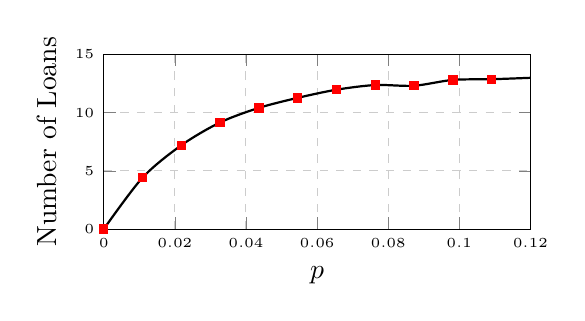
\begin{tikzpicture}
        \begin{axis}[
          ylabel={Number of Loans},
          ymin=0,
          xmin=0, xmax=0.12,
          width=7cm, height=3.8cm,
          ymax=15,
        ]
          \addplot[only marks, mark=square*, red] coordinates { (1e-05,0.00) (0.01091909090909091,4.42) (0.02182818181818182,7.20) (0.03273727272727273,9.16) (0.04364636363636364,10.41) (0.05455545454545455,11.27) (0.06546454545454546,11.97) (0.07637363636363637,12.37) (0.08728272727272728,12.31) (0.09819181818181819,12.81) (0.1091009090909091,12.87) (0.12001,12.99) };
          \addplot[black line] coordinates { (1e-05,0.00) (0.01091909090909091,4.42) (0.02182818181818182,7.20) (0.03273727272727273,9.16) (0.04364636363636364,10.41) (0.05455545454545455,11.27) (0.06546454545454546,11.97) (0.07637363636363637,12.37) (0.08728272727272728,12.31) (0.09819181818181819,12.81) (0.1091009090909091,12.87) (0.12001,12.99) };
        \end{axis}
        \end{tikzpicture}
      \end{figure}
      \vspace{-0.3cm}
      \tiny\renewcommand{\arraystretch}{0.85}\setlength{\tabcolsep}{2pt}
      \centering
      \begin{tabular}{lr}
        \toprule
        $p$ & Val. \\
        \midrule
          0.00001 & 0.00 \\
          0.011 & 4.42 \\
          0.022 & 7.20 \\
          0.033 & 9.16 \\
          0.044 & 10.41 \\
          0.055 & 11.27 \\
          0.065 & 11.97 \\
          0.076 & 12.37 \\
          0.087 & 12.31 \\
          0.098 & 12.81 \\
          0.109 & 12.87 \\
          0.120 & 12.99 \\
        \bottomrule
      \end{tabular}
    \end{column}
  \end{columns}
\end{frame}

\begin{frame}{Leverage }
  \begin{columns}[T]
    \begin{column}{0.4\textwidth}
      \centering
      \small $p=[0 .. 1]$\\
      \begin{figure}
        \centering
        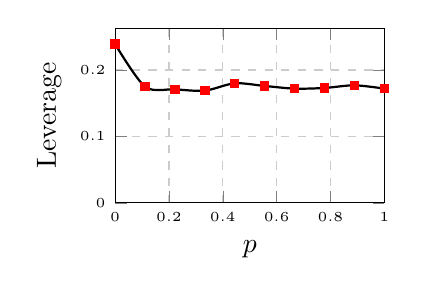
\begin{tikzpicture}
        \begin{axis}[
          ylabel={Leverage},
          ymin=0,
          xmin=0, xmax=1.0,
          width=5cm, height=3.8cm,
        ]
          \addplot[only marks, mark=square*, red] coordinates { (1e-05,0.239) (0.11112,0.175) (0.22223,0.171) (0.33334,0.169) (0.44445,0.180) (0.5555599999999999,0.176) (0.66667,0.172) (0.7777799999999999,0.173) (0.88889,0.177) (1.0,0.172) };
          \addplot[black line] coordinates { (1e-05,0.239) (0.11112,0.175) (0.22223,0.171) (0.33334,0.169) (0.44445,0.180) (0.5555599999999999,0.176) (0.66667,0.172) (0.7777799999999999,0.173) (0.88889,0.177) (1.0,0.172) };
        \end{axis}
        \end{tikzpicture}
      \end{figure}
      \vspace{-0.3cm}
      \tiny\renewcommand{\arraystretch}{0.85}\setlength{\tabcolsep}{2pt}
      \centering
      \begin{tabular}{lr}
        \toprule
        $p$ & Val. \\
        \midrule
          0.00001 & 0.239 \\
          0.111 & 0.175 \\
          0.222 & 0.171 \\
          0.333 & 0.169 \\
          0.444 & 0.180 \\
          0.556 & 0.176 \\
          0.667 & 0.172 \\
          0.778 & 0.173 \\
          0.889 & 0.177 \\
          1.000 & 0.172 \\
        \bottomrule
      \end{tabular}
    \end{column}
    \begin{column}{0.6\textwidth}
      \centering
      \small $p=[0 .. 0.12]$\\
      \begin{figure}
        \centering
        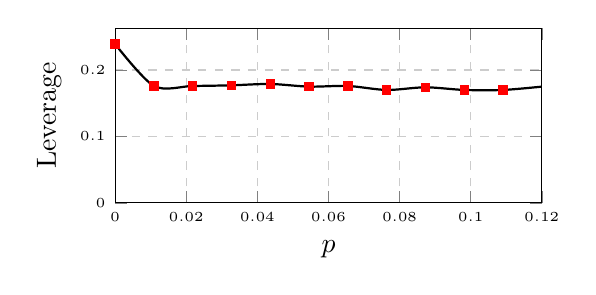
\begin{tikzpicture}
        \begin{axis}[
          ylabel={Leverage},
          ymin=0,
          xmin=0, xmax=0.12,
          width=7cm, height=3.8cm,
        ]
          \addplot[only marks, mark=square*, red] coordinates { (1e-05,0.239) (0.01091909090909091,0.176) (0.02182818181818182,0.176) (0.03273727272727273,0.177) (0.04364636363636364,0.179) (0.05455545454545455,0.175) (0.06546454545454546,0.176) (0.07637363636363637,0.170) (0.08728272727272728,0.174) (0.09819181818181819,0.170) (0.1091009090909091,0.170) (0.12001,0.175) };
          \addplot[black line] coordinates { (1e-05,0.239) (0.01091909090909091,0.176) (0.02182818181818182,0.176) (0.03273727272727273,0.177) (0.04364636363636364,0.179) (0.05455545454545455,0.175) (0.06546454545454546,0.176) (0.07637363636363637,0.170) (0.08728272727272728,0.174) (0.09819181818181819,0.170) (0.1091009090909091,0.170) (0.12001,0.175) };
        \end{axis}
        \end{tikzpicture}
      \end{figure}
      \vspace{-0.3cm}
      \tiny\renewcommand{\arraystretch}{0.85}\setlength{\tabcolsep}{2pt}
      \centering
      \begin{tabular}{lr}
        \toprule
        $p$ & Val. \\
        \midrule
          0.00001 & 0.239 \\
          0.011 & 0.176 \\
          0.022 & 0.176 \\
          0.033 & 0.177 \\
          0.044 & 0.179 \\
          0.055 & 0.175 \\
          0.065 & 0.176 \\
          0.076 & 0.170 \\
          0.087 & 0.174 \\
          0.098 & 0.170 \\
          0.109 & 0.170 \\
          0.120 & 0.175 \\
        \bottomrule
      \end{tabular}
    \end{column}
  \end{columns}
\end{frame}

\begin{frame}{Liquidity }
  \begin{columns}[T]
    \begin{column}{0.4\textwidth}
      \centering
      \small $p=[0 .. 1]$\\
      \begin{figure}
        \centering
        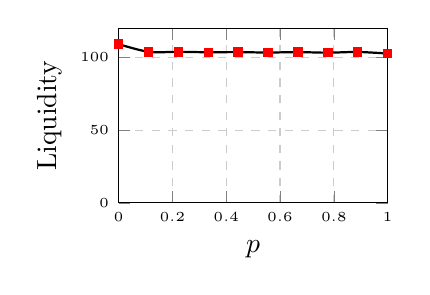
\begin{tikzpicture}
        \begin{axis}[
          ylabel={Liquidity},
          ymin=0,
          xmin=0, xmax=1.0,
          width=5cm, height=3.8cm,
        ]
          \addplot[only marks, mark=square*, red] coordinates { (1e-05,109.2) (0.11112,103.9) (0.22223,103.9) (0.33334,103.6) (0.44445,103.7) (0.5555599999999999,103.4) (0.66667,103.7) (0.7777799999999999,103.3) (0.88889,103.8) (1.0,102.7) };
          \addplot[black line] coordinates { (1e-05,109.2) (0.11112,103.9) (0.22223,103.9) (0.33334,103.6) (0.44445,103.7) (0.5555599999999999,103.4) (0.66667,103.7) (0.7777799999999999,103.3) (0.88889,103.8) (1.0,102.7) };
        \end{axis}
        \end{tikzpicture}
      \end{figure}
      \vspace{-0.3cm}
      \tiny\renewcommand{\arraystretch}{0.85}\setlength{\tabcolsep}{2pt}
      \centering
      \begin{tabular}{lr}
        \toprule
        $p$ & Val. \\
        \midrule
          0.00001 & 109.2 \\
          0.111 & 103.9 \\
          0.222 & 103.9 \\
          0.333 & 103.6 \\
          0.444 & 103.7 \\
          0.556 & 103.4 \\
          0.667 & 103.7 \\
          0.778 & 103.3 \\
          0.889 & 103.8 \\
          1.000 & 102.7 \\
        \bottomrule
      \end{tabular}
    \end{column}
    \begin{column}{0.6\textwidth}
      \centering
      \small $p=[0 .. 0.12]$\\
      \begin{figure}
        \centering
        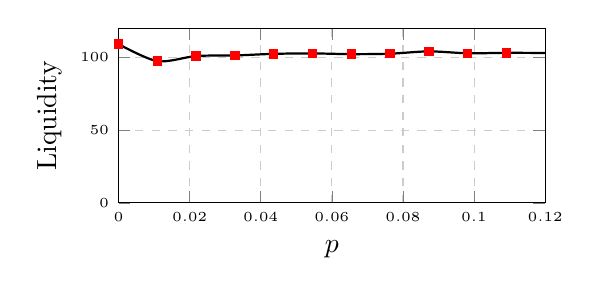
\begin{tikzpicture}
        \begin{axis}[
          ylabel={Liquidity},
          ymin=0,
          xmin=0, xmax=0.12,
          width=7cm, height=3.8cm,
        ]
          \addplot[only marks, mark=square*, red] coordinates { (1e-05,109.2) (0.01091909090909091,97.5) (0.02182818181818182,101.0) (0.03273727272727273,101.4) (0.04364636363636364,102.5) (0.05455545454545455,102.8) (0.06546454545454546,102.3) (0.07637363636363637,102.6) (0.08728272727272728,104.2) (0.09819181818181819,102.9) (0.1091009090909091,103.2) (0.12001,103.1) };
          \addplot[black line] coordinates { (1e-05,109.2) (0.01091909090909091,97.5) (0.02182818181818182,101.0) (0.03273727272727273,101.4) (0.04364636363636364,102.5) (0.05455545454545455,102.8) (0.06546454545454546,102.3) (0.07637363636363637,102.6) (0.08728272727272728,104.2) (0.09819181818181819,102.9) (0.1091009090909091,103.2) (0.12001,103.1) };
        \end{axis}
        \end{tikzpicture}
      \end{figure}
      \vspace{-0.3cm}
      \tiny\renewcommand{\arraystretch}{0.85}\setlength{\tabcolsep}{2pt}
      \centering
      \begin{tabular}{lr}
        \toprule
        $p$ & Val. \\
        \midrule
          0.00001 & 109.2 \\
          0.011 & 97.5 \\
          0.022 & 101.0 \\
          0.033 & 101.4 \\
          0.044 & 102.5 \\
          0.055 & 102.8 \\
          0.065 & 102.3 \\
          0.076 & 102.6 \\
          0.087 & 104.2 \\
          0.098 & 102.9 \\
          0.109 & 103.2 \\
          0.120 & 103.1 \\
        \bottomrule
      \end{tabular}
    \end{column}
  \end{columns}
\end{frame}

\begin{frame}{Deposits }
  \begin{columns}[T]
    \begin{column}{0.4\textwidth}
      \centering
      \small $p=[0 .. 1]$\\
      \begin{figure}
        \centering
        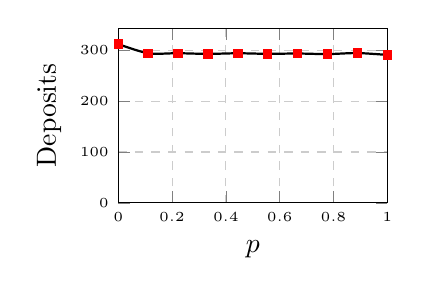
\begin{tikzpicture}
        \begin{axis}[
          ylabel={Deposits},
          ymin=0,
          xmin=0, xmax=1.0,
          width=5cm, height=3.8cm,
        ]
          \addplot[only marks, mark=square*, red] coordinates { (1e-05,312.0) (0.11112,294.1) (0.22223,294.1) (0.33334,292.8) (0.44445,294.0) (0.5555599999999999,292.9) (0.66667,293.5) (0.7777799999999999,292.4) (0.88889,294.4) (1.0,290.7) };
          \addplot[black line] coordinates { (1e-05,312.0) (0.11112,294.1) (0.22223,294.1) (0.33334,292.8) (0.44445,294.0) (0.5555599999999999,292.9) (0.66667,293.5) (0.7777799999999999,292.4) (0.88889,294.4) (1.0,290.7) };
        \end{axis}
        \end{tikzpicture}
      \end{figure}
      \vspace{-0.3cm}
      \tiny\renewcommand{\arraystretch}{0.85}\setlength{\tabcolsep}{2pt}
      \centering
      \begin{tabular}{lr}
        \toprule
        $p$ & Val. \\
        \midrule
          0.00001 & 312.0 \\
          0.111 & 294.1 \\
          0.222 & 294.1 \\
          0.333 & 292.8 \\
          0.444 & 294.0 \\
          0.556 & 292.9 \\
          0.667 & 293.5 \\
          0.778 & 292.4 \\
          0.889 & 294.4 \\
          1.000 & 290.7 \\
        \bottomrule
      \end{tabular}
    \end{column}
    \begin{column}{0.6\textwidth}
      \centering
      \small $p=[0 .. 0.12]$\\
      \begin{figure}
        \centering
        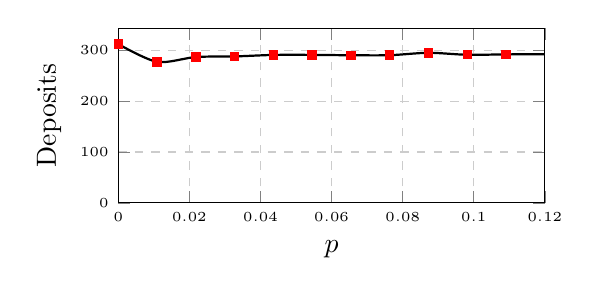
\begin{tikzpicture}
        \begin{axis}[
          ylabel={Deposits},
          ymin=0,
          xmin=0, xmax=0.12,
          width=7cm, height=3.8cm,
        ]
          \addplot[only marks, mark=square*, red] coordinates { (1e-05,312.2) (0.01091909090909091,277.4) (0.02182818181818182,286.8) (0.03273727272727273,288.0) (0.04364636363636364,290.9) (0.05455545454545455,291.0) (0.06546454545454546,290.3) (0.07637363636363637,290.4) (0.08728272727272728,295.1) (0.09819181818181819,291.2) (0.1091009090909091,292.0) (0.12001,292.1) };
          \addplot[black line] coordinates { (1e-05,312.2) (0.01091909090909091,277.4) (0.02182818181818182,286.8) (0.03273727272727273,288.0) (0.04364636363636364,290.9) (0.05455545454545455,291.0) (0.06546454545454546,290.3) (0.07637363636363637,290.4) (0.08728272727272728,295.1) (0.09819181818181819,291.2) (0.1091009090909091,292.0) (0.12001,292.1) };
        \end{axis}
        \end{tikzpicture}
      \end{figure}
      \vspace{-0.3cm}
      \tiny\renewcommand{\arraystretch}{0.85}\setlength{\tabcolsep}{2pt}
      \centering
      \begin{tabular}{lr}
        \toprule
        $p$ & Val. \\
        \midrule
          0.00001 & 312.2 \\
          0.011 & 277.4 \\
          0.022 & 286.8 \\
          0.033 & 288.0 \\
          0.044 & 290.9 \\
          0.055 & 291.0 \\
          0.065 & 290.3 \\
          0.076 & 290.4 \\
          0.087 & 295.1 \\
          0.098 & 291.2 \\
          0.109 & 292.0 \\
          0.120 & 292.1 \\
        \bottomrule
      \end{tabular}
    \end{column}
  \end{columns}
\end{frame}

\begin{frame}{Market Power ($\psi$) }
  \begin{columns}[T]
    \begin{column}{0.4\textwidth}
      \centering
      \small $p=[0 .. 1]$\\
      \begin{figure}
        \centering
        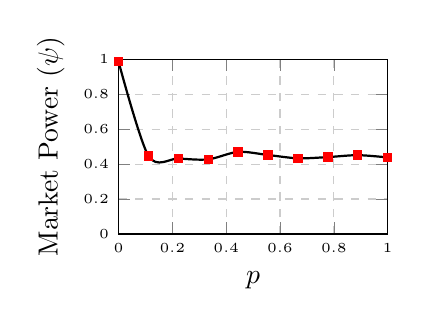
\begin{tikzpicture}
        \begin{axis}[
          ylabel={Market Power ($\psi$)},
          ymin=0,
          xmin=0, xmax=1.0,
          width=5cm, height=3.8cm,
          ymax=1,
        ]
          \addplot[only marks, mark=square*, red] coordinates { (1e-05,0.987) (0.11112,0.447) (0.22223,0.432) (0.33334,0.427) (0.44445,0.470) (0.5555599999999999,0.452) (0.66667,0.433) (0.7777799999999999,0.440) (0.88889,0.451) (1.0,0.438) };
          \addplot[black line] coordinates { (1e-05,0.987) (0.11112,0.447) (0.22223,0.432) (0.33334,0.427) (0.44445,0.470) (0.5555599999999999,0.452) (0.66667,0.433) (0.7777799999999999,0.440) (0.88889,0.451) (1.0,0.438) };
        \end{axis}
        \end{tikzpicture}
      \end{figure}
      \vspace{-0.3cm}
      \tiny\renewcommand{\arraystretch}{0.85}\setlength{\tabcolsep}{2pt}
      \centering
      \begin{tabular}{lr}
        \toprule
        $p$ & Val. \\
        \midrule
          0.00001 & 0.987 \\
          0.111 & 0.447 \\
          0.222 & 0.432 \\
          0.333 & 0.427 \\
          0.444 & 0.470 \\
          0.556 & 0.452 \\
          0.667 & 0.433 \\
          0.778 & 0.440 \\
          0.889 & 0.451 \\
          1.000 & 0.438 \\
        \bottomrule
      \end{tabular}
    \end{column}
    \begin{column}{0.6\textwidth}
      \centering
      \small $p=[0 .. 0.12]$\\
      \begin{figure}
        \centering
        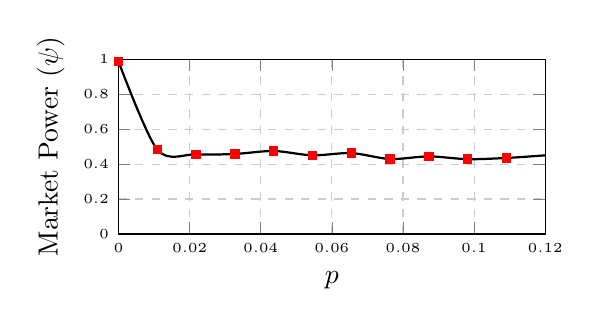
\begin{tikzpicture}
        \begin{axis}[
          ylabel={Market Power ($\psi$)},
          ymin=0,
          xmin=0, xmax=0.12,
          width=7cm, height=3.8cm,
          ymax=1,
        ]
          \addplot[only marks, mark=square*, red] coordinates { (1e-05,0.987) (0.01091909090909091,0.482) (0.02182818181818182,0.456) (0.03273727272727273,0.458) (0.04364636363636364,0.475) (0.05455545454545455,0.450) (0.06546454545454546,0.463) (0.07637363636363637,0.429) (0.08728272727272728,0.444) (0.09819181818181819,0.428) (0.1091009090909091,0.435) (0.12001,0.450) };
          \addplot[black line] coordinates { (1e-05,0.987) (0.01091909090909091,0.482) (0.02182818181818182,0.456) (0.03273727272727273,0.458) (0.04364636363636364,0.475) (0.05455545454545455,0.450) (0.06546454545454546,0.463) (0.07637363636363637,0.429) (0.08728272727272728,0.444) (0.09819181818181819,0.428) (0.1091009090909091,0.435) (0.12001,0.450) };
        \end{axis}
        \end{tikzpicture}
      \end{figure}
      \vspace{-0.3cm}
      \tiny\renewcommand{\arraystretch}{0.85}\setlength{\tabcolsep}{2pt}
      \centering
      \begin{tabular}{lr}
        \toprule
        $p$ & Val. \\
        \midrule
          0.00001 & 0.987 \\
          0.011 & 0.482 \\
          0.022 & 0.456 \\
          0.033 & 0.458 \\
          0.044 & 0.475 \\
          0.055 & 0.450 \\
          0.065 & 0.463 \\
          0.076 & 0.429 \\
          0.087 & 0.444 \\
          0.098 & 0.428 \\
          0.109 & 0.435 \\
          0.120 & 0.450 \\
        \bottomrule
      \end{tabular}
    \end{column}
  \end{columns}
\end{frame}

\begin{frame}{Interest Rate ($ir$) }
  \begin{columns}[T]
    \begin{column}{0.4\textwidth}
      \centering
      \small $p=[0 .. 1]$\\
      \begin{figure}
        \centering
        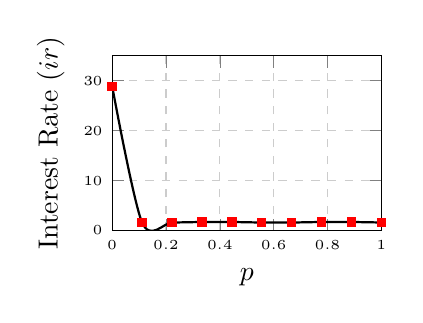
\begin{tikzpicture}
        \begin{axis}[
          ylabel={Interest Rate ($ir$)},
          ymin=0,
          xmin=0, xmax=1.0,
          width=5cm, height=3.8cm,
          ymax=35,
        ]
          \addplot[only marks, mark=square*, red] coordinates { (1e-05,28.9) (0.11112,1.6) (0.22223,1.6) (0.33334,1.7) (0.44445,1.7) (0.5555599999999999,1.6) (0.66667,1.6) (0.7777799999999999,1.7) (0.88889,1.7) (1.0,1.6) };
          \addplot[black line] coordinates { (1e-05,28.9) (0.11112,1.6) (0.22223,1.6) (0.33334,1.7) (0.44445,1.7) (0.5555599999999999,1.6) (0.66667,1.6) (0.7777799999999999,1.7) (0.88889,1.7) (1.0,1.6) };
        \end{axis}
        \end{tikzpicture}
      \end{figure}
      \vspace{-0.3cm}
      \tiny\renewcommand{\arraystretch}{0.85}\setlength{\tabcolsep}{2pt}
      \centering
      \begin{tabular}{lr}
        \toprule
        $p$ & Val. \\
        \midrule
          0.00001 & 28.9 \\
          0.111 & 1.6 \\
          0.222 & 1.6 \\
          0.333 & 1.7 \\
          0.444 & 1.7 \\
          0.556 & 1.6 \\
          0.667 & 1.6 \\
          0.778 & 1.7 \\
          0.889 & 1.7 \\
          1.000 & 1.6 \\
        \bottomrule
      \end{tabular}
    \end{column}
    \begin{column}{0.6\textwidth}
      \centering
      \small $p=[0 .. 0.12]$\\
      \begin{figure}
        \centering
        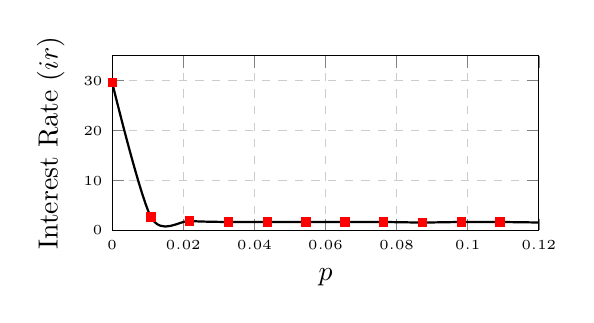
\begin{tikzpicture}
        \begin{axis}[
          ylabel={Interest Rate ($ir$)},
          ymin=0,
          xmin=0, xmax=0.12,
          width=7cm, height=3.8cm,
          ymax=35,
        ]
          \addplot[only marks, mark=square*, red] coordinates { (1e-05,29.6) (0.01091909090909091,2.7) (0.02182818181818182,1.9) (0.03273727272727273,1.7) (0.04364636363636364,1.7) (0.05455545454545455,1.7) (0.06546454545454546,1.7) (0.07637363636363637,1.7) (0.08728272727272728,1.6) (0.09819181818181819,1.7) (0.1091009090909091,1.7) (0.12001,1.6) };
          \addplot[black line] coordinates { (1e-05,29.6) (0.01091909090909091,2.7) (0.02182818181818182,1.9) (0.03273727272727273,1.7) (0.04364636363636364,1.7) (0.05455545454545455,1.7) (0.06546454545454546,1.7) (0.07637363636363637,1.7) (0.08728272727272728,1.6) (0.09819181818181819,1.7) (0.1091009090909091,1.7) (0.12001,1.6) };
        \end{axis}
        \end{tikzpicture}
      \end{figure}
      \vspace{-0.3cm}
      \tiny\renewcommand{\arraystretch}{0.85}\setlength{\tabcolsep}{2pt}
      \centering
      \begin{tabular}{lr}
        \toprule
        $p$ & Val. \\
        \midrule
          0.00001 & 29.6 \\
          0.011 & 2.7 \\
          0.022 & 1.9 \\
          0.033 & 1.7 \\
          0.044 & 1.7 \\
          0.055 & 1.7 \\
          0.065 & 1.7 \\
          0.076 & 1.7 \\
          0.087 & 1.6 \\
          0.098 & 1.7 \\
          0.109 & 1.7 \\
          0.120 & 1.6 \\
        \bottomrule
      \end{tabular}
    \end{column}
  \end{columns}
\end{frame}

\begin{frame}{Prob. of Bankruptcy ($p_b$) }
  \begin{columns}[T]
    \begin{column}{0.4\textwidth}
      \centering
      \small $p=[0 .. 1]$\\
      \begin{figure}
        \centering
        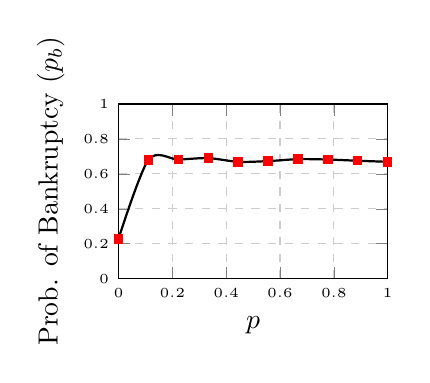
\begin{tikzpicture}
        \begin{axis}[
          ylabel={Prob. of Bankruptcy ($p_b$)},
          ymin=0,
          xmin=0, xmax=1.0,
          width=5cm, height=3.8cm,
          ymax=1,
        ]
          \addplot[only marks, mark=square*, red] coordinates { (1e-05,0.228) (0.11112,0.680) (0.22223,0.682) (0.33334,0.690) (0.44445,0.669) (0.5555599999999999,0.673) (0.66667,0.684) (0.7777799999999999,0.682) (0.88889,0.675) (1.0,0.669) };
          \addplot[black line] coordinates { (1e-05,0.228) (0.11112,0.680) (0.22223,0.682) (0.33334,0.690) (0.44445,0.669) (0.5555599999999999,0.673) (0.66667,0.684) (0.7777799999999999,0.682) (0.88889,0.675) (1.0,0.669) };
        \end{axis}
        \end{tikzpicture}
      \end{figure}
      \vspace{-0.3cm}
      \tiny\renewcommand{\arraystretch}{0.85}\setlength{\tabcolsep}{2pt}
      \centering
      \begin{tabular}{lr}
        \toprule
        $p$ & Val. \\
        \midrule
          0.00001 & 0.228 \\
          0.111 & 0.680 \\
          0.222 & 0.682 \\
          0.333 & 0.690 \\
          0.444 & 0.669 \\
          0.556 & 0.673 \\
          0.667 & 0.684 \\
          0.778 & 0.682 \\
          0.889 & 0.675 \\
          1.000 & 0.669 \\
        \bottomrule
      \end{tabular}
    \end{column}
    \begin{column}{0.6\textwidth}
      \centering
      \small $p=[0 .. 0.12]$\\
      \begin{figure}
        \centering
        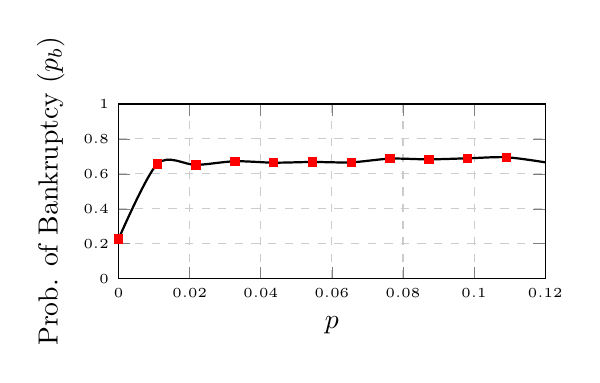
\begin{tikzpicture}
        \begin{axis}[
          ylabel={Prob. of Bankruptcy ($p_b$)},
          ymin=0,
          xmin=0, xmax=0.12,
          width=7cm, height=3.8cm,
          ymax=1,
        ]
          \addplot[only marks, mark=square*, red] coordinates { (1e-05,0.227) (0.01091909090909091,0.657) (0.02182818181818182,0.651) (0.03273727272727273,0.672) (0.04364636363636364,0.664) (0.05455545454545455,0.668) (0.06546454545454546,0.666) (0.07637363636363637,0.687) (0.08728272727272728,0.683) (0.09819181818181819,0.689) (0.1091009090909091,0.695) (0.12001,0.666) };
          \addplot[black line] coordinates { (1e-05,0.227) (0.01091909090909091,0.657) (0.02182818181818182,0.651) (0.03273727272727273,0.672) (0.04364636363636364,0.664) (0.05455545454545455,0.668) (0.06546454545454546,0.666) (0.07637363636363637,0.687) (0.08728272727272728,0.683) (0.09819181818181819,0.689) (0.1091009090909091,0.695) (0.12001,0.666) };
        \end{axis}
        \end{tikzpicture}
      \end{figure}
      \vspace{-0.3cm}
      \tiny\renewcommand{\arraystretch}{0.85}\setlength{\tabcolsep}{2pt}
      \centering
      \begin{tabular}{lr}
        \toprule
        $p$ & Val. \\
        \midrule
          0.00001 & 0.227 \\
          0.011 & 0.657 \\
          0.022 & 0.651 \\
          0.033 & 0.672 \\
          0.044 & 0.664 \\
          0.055 & 0.668 \\
          0.065 & 0.666 \\
          0.076 & 0.687 \\
          0.087 & 0.683 \\
          0.098 & 0.689 \\
          0.109 & 0.695 \\
          0.120 & 0.666 \\
        \bottomrule
      \end{tabular}
    \end{column}
  \end{columns}
\end{frame}

\begin{frame}{Equity}
  \begin{columns}[T]
    \begin{column}{0.4\textwidth}
      \centering
      \small $p=[0 .. 1]$\\
      \begin{figure}
        \centering
        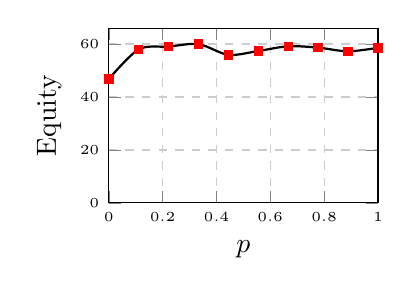
\begin{tikzpicture}
        \begin{axis}[
          ylabel={Equity},
          ymin=0,
          xmin=0, xmax=1.0,
          width=5cm, height=3.8cm,
        ]
          \addplot[only marks, mark=square*, red] coordinates { (1e-05,46.79) (0.11112,58.01) (0.22223,59.03) (0.33334,59.97) (0.44445,55.91) (0.5555599999999999,57.37) (0.66667,59.16) (0.7777799999999999,58.64) (0.88889,57.24) (1.0,58.57) };
          \addplot[black line] coordinates { (1e-05,46.79) (0.11112,58.01) (0.22223,59.03) (0.33334,59.97) (0.44445,55.91) (0.5555599999999999,57.37) (0.66667,59.16) (0.7777799999999999,58.64) (0.88889,57.24) (1.0,58.57) };
        \end{axis}
        \end{tikzpicture}
      \end{figure}
      \vspace{-0.3cm}
      \tiny\renewcommand{\arraystretch}{0.85}\setlength{\tabcolsep}{2pt}
      \centering
      \begin{tabular}{lr}
        \toprule
        $p$ & Val. \\
        \midrule
          0.00001 & 46.79 \\
          0.111 & 58.01 \\
          0.222 & 59.03 \\
          0.333 & 59.97 \\
          0.444 & 55.91 \\
          0.556 & 57.37 \\
          0.667 & 59.16 \\
          0.778 & 58.64 \\
          0.889 & 57.24 \\
          1.000 & 58.57 \\
        \bottomrule
      \end{tabular}
    \end{column}
    \begin{column}{0.6\textwidth}
      \centering
      \small $p=[0 .. 0.12]$\\
      \begin{figure}
        \centering
        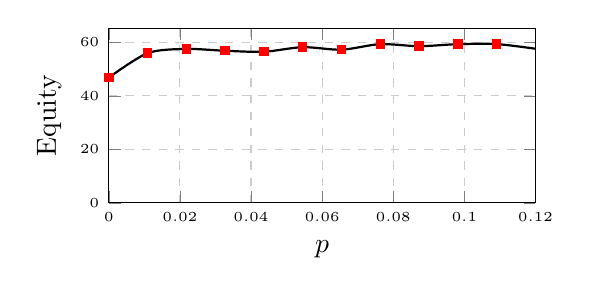
\begin{tikzpicture}
        \begin{axis}[
          ylabel={Equity},
          ymin=0,
          xmin=0, xmax=0.12,
          width=7cm, height=3.8cm,
        ]
          \addplot[only marks, mark=square*, red] coordinates { (1e-05,46.81) (0.01091909090909091,55.95) (0.02182818181818182,57.52) (0.03273727272727273,56.84) (0.04364636363636364,56.48) (0.05455545454545455,58.18) (0.06546454545454546,57.25) (0.07637363636363637,59.31) (0.08728272727272728,58.55) (0.09819181818181819,59.31) (0.1091009090909091,59.33) (0.12001,57.59) };
          \addplot[black line] coordinates { (1e-05,46.81) (0.01091909090909091,55.95) (0.02182818181818182,57.52) (0.03273727272727273,56.84) (0.04364636363636364,56.48) (0.05455545454545455,58.18) (0.06546454545454546,57.25) (0.07637363636363637,59.31) (0.08728272727272728,58.55) (0.09819181818181819,59.31) (0.1091009090909091,59.33) (0.12001,57.59) };
        \end{axis}
        \end{tikzpicture}
      \end{figure}
      \vspace{-0.3cm}
      \tiny\renewcommand{\arraystretch}{0.85}\setlength{\tabcolsep}{2pt}
      \centering
      \begin{tabular}{lr}
        \toprule
        $p$ & Val. \\
        \midrule
          0.00001 & 46.81 \\
          0.011 & 55.95 \\
          0.022 & 57.52 \\
          0.033 & 56.84 \\
          0.044 & 56.48 \\
          0.055 & 58.18 \\
          0.065 & 57.25 \\
          0.076 & 59.31 \\
          0.087 & 58.55 \\
          0.098 & 59.31 \\
          0.109 & 59.33 \\
          0.120 & 57.59 \\
        \bottomrule
      \end{tabular}
    \end{column}
  \end{columns}
\end{frame}

\end{document}